% Options for packages loaded elsewhere
\PassOptionsToPackage{unicode}{hyperref}
\PassOptionsToPackage{hyphens}{url}
%
\documentclass[
]{book}
\usepackage{amsmath,amssymb}
\usepackage{lmodern}
\usepackage{iftex}
\ifPDFTeX
  \usepackage[T1]{fontenc}
  \usepackage[utf8]{inputenc}
  \usepackage{textcomp} % provide euro and other symbols
\else % if luatex or xetex
  \usepackage{unicode-math}
  \defaultfontfeatures{Scale=MatchLowercase}
  \defaultfontfeatures[\rmfamily]{Ligatures=TeX,Scale=1}
\fi
% Use upquote if available, for straight quotes in verbatim environments
\IfFileExists{upquote.sty}{\usepackage{upquote}}{}
\IfFileExists{microtype.sty}{% use microtype if available
  \usepackage[]{microtype}
  \UseMicrotypeSet[protrusion]{basicmath} % disable protrusion for tt fonts
}{}
\makeatletter
\@ifundefined{KOMAClassName}{% if non-KOMA class
  \IfFileExists{parskip.sty}{%
    \usepackage{parskip}
  }{% else
    \setlength{\parindent}{0pt}
    \setlength{\parskip}{6pt plus 2pt minus 1pt}}
}{% if KOMA class
  \KOMAoptions{parskip=half}}
\makeatother
\usepackage{xcolor}
\IfFileExists{xurl.sty}{\usepackage{xurl}}{} % add URL line breaks if available
\IfFileExists{bookmark.sty}{\usepackage{bookmark}}{\usepackage{hyperref}}
\hypersetup{
  pdftitle={NLP Galore},
  pdfauthor={Various Sources},
  hidelinks,
  pdfcreator={LaTeX via pandoc}}
\urlstyle{same} % disable monospaced font for URLs
\usepackage{color}
\usepackage{fancyvrb}
\newcommand{\VerbBar}{|}
\newcommand{\VERB}{\Verb[commandchars=\\\{\}]}
\DefineVerbatimEnvironment{Highlighting}{Verbatim}{commandchars=\\\{\}}
% Add ',fontsize=\small' for more characters per line
\usepackage{framed}
\definecolor{shadecolor}{RGB}{248,248,248}
\newenvironment{Shaded}{\begin{snugshade}}{\end{snugshade}}
\newcommand{\AlertTok}[1]{\textcolor[rgb]{0.94,0.16,0.16}{#1}}
\newcommand{\AnnotationTok}[1]{\textcolor[rgb]{0.56,0.35,0.01}{\textbf{\textit{#1}}}}
\newcommand{\AttributeTok}[1]{\textcolor[rgb]{0.77,0.63,0.00}{#1}}
\newcommand{\BaseNTok}[1]{\textcolor[rgb]{0.00,0.00,0.81}{#1}}
\newcommand{\BuiltInTok}[1]{#1}
\newcommand{\CharTok}[1]{\textcolor[rgb]{0.31,0.60,0.02}{#1}}
\newcommand{\CommentTok}[1]{\textcolor[rgb]{0.56,0.35,0.01}{\textit{#1}}}
\newcommand{\CommentVarTok}[1]{\textcolor[rgb]{0.56,0.35,0.01}{\textbf{\textit{#1}}}}
\newcommand{\ConstantTok}[1]{\textcolor[rgb]{0.00,0.00,0.00}{#1}}
\newcommand{\ControlFlowTok}[1]{\textcolor[rgb]{0.13,0.29,0.53}{\textbf{#1}}}
\newcommand{\DataTypeTok}[1]{\textcolor[rgb]{0.13,0.29,0.53}{#1}}
\newcommand{\DecValTok}[1]{\textcolor[rgb]{0.00,0.00,0.81}{#1}}
\newcommand{\DocumentationTok}[1]{\textcolor[rgb]{0.56,0.35,0.01}{\textbf{\textit{#1}}}}
\newcommand{\ErrorTok}[1]{\textcolor[rgb]{0.64,0.00,0.00}{\textbf{#1}}}
\newcommand{\ExtensionTok}[1]{#1}
\newcommand{\FloatTok}[1]{\textcolor[rgb]{0.00,0.00,0.81}{#1}}
\newcommand{\FunctionTok}[1]{\textcolor[rgb]{0.00,0.00,0.00}{#1}}
\newcommand{\ImportTok}[1]{#1}
\newcommand{\InformationTok}[1]{\textcolor[rgb]{0.56,0.35,0.01}{\textbf{\textit{#1}}}}
\newcommand{\KeywordTok}[1]{\textcolor[rgb]{0.13,0.29,0.53}{\textbf{#1}}}
\newcommand{\NormalTok}[1]{#1}
\newcommand{\OperatorTok}[1]{\textcolor[rgb]{0.81,0.36,0.00}{\textbf{#1}}}
\newcommand{\OtherTok}[1]{\textcolor[rgb]{0.56,0.35,0.01}{#1}}
\newcommand{\PreprocessorTok}[1]{\textcolor[rgb]{0.56,0.35,0.01}{\textit{#1}}}
\newcommand{\RegionMarkerTok}[1]{#1}
\newcommand{\SpecialCharTok}[1]{\textcolor[rgb]{0.00,0.00,0.00}{#1}}
\newcommand{\SpecialStringTok}[1]{\textcolor[rgb]{0.31,0.60,0.02}{#1}}
\newcommand{\StringTok}[1]{\textcolor[rgb]{0.31,0.60,0.02}{#1}}
\newcommand{\VariableTok}[1]{\textcolor[rgb]{0.00,0.00,0.00}{#1}}
\newcommand{\VerbatimStringTok}[1]{\textcolor[rgb]{0.31,0.60,0.02}{#1}}
\newcommand{\WarningTok}[1]{\textcolor[rgb]{0.56,0.35,0.01}{\textbf{\textit{#1}}}}
\usepackage{longtable,booktabs,array}
\usepackage{calc} % for calculating minipage widths
% Correct order of tables after \paragraph or \subparagraph
\usepackage{etoolbox}
\makeatletter
\patchcmd\longtable{\par}{\if@noskipsec\mbox{}\fi\par}{}{}
\makeatother
% Allow footnotes in longtable head/foot
\IfFileExists{footnotehyper.sty}{\usepackage{footnotehyper}}{\usepackage{footnote}}
\makesavenoteenv{longtable}
\usepackage{graphicx}
\makeatletter
\def\maxwidth{\ifdim\Gin@nat@width>\linewidth\linewidth\else\Gin@nat@width\fi}
\def\maxheight{\ifdim\Gin@nat@height>\textheight\textheight\else\Gin@nat@height\fi}
\makeatother
% Scale images if necessary, so that they will not overflow the page
% margins by default, and it is still possible to overwrite the defaults
% using explicit options in \includegraphics[width, height, ...]{}
\setkeys{Gin}{width=\maxwidth,height=\maxheight,keepaspectratio}
% Set default figure placement to htbp
\makeatletter
\def\fps@figure{htbp}
\makeatother
\usepackage[normalem]{ulem}
% Avoid problems with \sout in headers with hyperref
\pdfstringdefDisableCommands{\renewcommand{\sout}{}}
\setlength{\emergencystretch}{3em} % prevent overfull lines
\providecommand{\tightlist}{%
  \setlength{\itemsep}{0pt}\setlength{\parskip}{0pt}}
\setcounter{secnumdepth}{5}
\usepackage{booktabs}
\ifLuaTeX
  \usepackage{selnolig}  % disable illegal ligatures
\fi
\usepackage[]{natbib}
\bibliographystyle{plainnat}

\title{NLP Galore}
\author{Various Sources}
\date{2022-08-28}

\begin{document}
\maketitle

{
\setcounter{tocdepth}{1}
\tableofcontents
}
\hypertarget{introduction}{%
\chapter{Introduction}\label{introduction}}

This handbook is about natural language processing for internal use only.

Please \textbf{do not} cite.

\hypertarget{part-basics-of-nlp}{%
\part*{BASICS OF NLP}\label{part-basics-of-nlp}}
\addcontentsline{toc}{part}{BASICS OF NLP}

\hypertarget{dictionary-based-methods}{%
\chapter{Dictionary-Based Methods}\label{dictionary-based-methods}}

\hypertarget{regression-based-methods}{%
\chapter{Regression-Based Methods}\label{regression-based-methods}}

Using document characteristics, these methods try to predict word frequencies in a given document. A natural way to model these relationships is using multinomial logistic regression; however, due to the large dimensionality of vocabularies, standard multinomial logistic regressions are not computationally feasible to implement. In recent years, econometric breakthroughs have led to the development of computationally feasible approximations of the ideal multinomial logit regression (Taddy, 2015).

These models have several applications. Firstly, the method tells us how the text depends on observed covariates. This is relevant in settings where the dependent variable is the text, e.g., political speeches. Secondly, once estimated, the model can be inverted to get predicted values of covariates using text as an input. This is particularly powerful for (i) nowcasting/forecasting and (ii) backcasting when data is missing (Kelly et al., 2021). For example, measurements of real activity such as GDP are only available with a lag and a quarterly frequency. However, economic media coverage is available in real-time and with low latency. Hence, it can be used to nowcast GDP. Similarly, when data have short histories, text can be used to backcast the data.

\hypertarget{challenges-of-having-text-as-the-dependent-variable}{%
\section{Challenges of having text as the dependent variable}\label{challenges-of-having-text-as-the-dependent-variable}}

The typical unit of analysis for text data is at the frequency of an n-gram in a given document, e.g., the number of times the word ``GDP'' turned up in a document. These frequencies are unordered uncategorical data, i.e., it is not obvious how to combine information that a document has ten mentions of the word ``GDP'' with six mentions of the word ``inflation.'' Hence, frequency counts are represented by a document \(i\) specific vectors that sit in \(\mathbf{c}_{i}\in\mathbb{R}^V\) where \(V\) is the number of unique n-grams in our sample. Note that \(V\) is extremely large in practice which is why machine learning methods are needed.

The go-to model to explain the document \(i\) specific count vector \(\mathbf{c}_{i}\) using variables \(\mathbf{v}_{i}\) would be a multinomial logit regression,
\[
\mathrm{p}\left(\mathbf{c}_{i} \mid \mathbf{v}_{i}, m_{i}\right) = \mathrm{MN}\left(\mathbf{c}_{i} ; \mathbf{q}_{i}, m_{i}\right) \text{ for } i=1 \ldots n
\]

\[
q_{i j} = \frac{e^{\eta_{i j}}}{\sum_{k=1}^{d} e^{\eta_{i k}}} \text { for } j=1 \ldots d
\]

\[
\eta_{i j} = \alpha_{j}+\mathbf{v}_{i}^{\prime} \varphi_{j}
\]

where \(q_{i j}\) is the n-gram's probability, \(m_i\) is the total number of n-grams in the document, and \((\alpha_j,\varphi_j)\) are the \(K+1\) n-gram specific parameters.

Given vocabularies often exceed \(10,000\) n-grams, estimating the model above with even just two covariates would mean estimating \(30,000+\) Parameters! The issue with standard multinomial estimation is that it cannot be parallelized; hence, estimating them for a large number of parameters is computationally prohibitive.

Multinomial logit regressions cannot be parallelized because the denominator of \(q_{ij}\) which depends on all the parameters in the model. Hence, to estimate the model, we need a parallelizable approximation. Taddy (2015) provided precisely such an approximation and used it to develop the distributed multinomial regression (DMR)

\hypertarget{distributed-multinomial-regressions-dmr}{%
\section{Distributed multinomial regressions (DMR)}\label{distributed-multinomial-regressions-dmr}}

A canonical relationship is that Multinomial distributions can be exactly decomposed into independent Poissons,
\[
\operatorname{MN}\left(\mathbf{c}_{i} ; \mathbf{q}_{i}, m_{i}\right)=\frac{\prod_{j} P_{o}\left(c_{i j} ; e^{\eta_{i j}}\right)}{P o\left(m_{i} ; \sum_{j=1}^{d} e^{\eta_{i j}}\right)}
\]
This decomposition does not solve the computation bottleneck since the denominator still depends on all parameters. However, Tadd (2015) used this decomposition to develop the following approximation,
\[
\mathrm{p}\left(\mathbf{c}_{i} \mid \mathbf{v}_{i}, m_{i}\right)=\mathrm{MN}\left(\mathbf{c}_{i} ; \mathbf{q}_{i}, m_{i}\right) \approx \prod_{j} \operatorname{Po}\left(c_{i j} ; m_{i} e^{\eta_{i j}}\right)
\]
Since this approximation doesn't depend on \(\sum_{j=1}^{d} e^{\eta_{i j}}\)It can be parallelized! Essentially, each n-gram's parameters are estimated separately using (shifted) Poisson regressions.

Taddy (2015) also developed a method for inverting the DMR so that post-estimation n-grams can be projected into covariates.

\hypertarget{extension-hurdle-dmr-hdmr}{%
\section{Extension: Hurdle DMR (HDMR)}\label{extension-hurdle-dmr-hdmr}}

In practice, while DMR works well for explaining strictly positive frequency counts (i.e., counts \textgreater{} 0), it performs poorly in explaining whether a word is used at all (i.e., count 0 or 1). Kelly et al.~(2021) developed the HDMR to simultaneously explain both the intensive margin (strictly positive frequency counts) and extensive margin (counts of zero and one) of word choice.

At a high level, the model combines a selection model with the DMR. The selection model approximates the extensive margin, and the DMR models the intensive margin.

Specifically, the selection model to include n-gram \(j\) in document \(i\) is standard,
\[
h_{i j}^{*}=\gamma_{i}+\kappa_{j}+\boldsymbol{w}_{i}^{\prime} \boldsymbol{\delta}_{j}+v_{i j}
\]
\[
h_{i j}=\mathbf{1}\left(h_{i j}^{*}>0\right)
\]

where \(\boldsymbol{w}_{i}\) are observed variables and \((\gamma_{i},\kappa_{j},\boldsymbol{\delta}_{j})\) Are parameters. And the count model has the following form,
\[
c_{i j}^{*} =\lambda\left(\mu_{i}+\alpha_{j}+\mathbf{v}_{i}^{\prime} \boldsymbol{\varphi}_{j}\right)+\varepsilon_{i j}
\]
\[
c_{i j} = \left(1+c_{i j}^{*}\right) h_{i j}
\]

where \(\boldsymbol{v}_{i}\) are observed variables and \((\mu_i,\alpha_j,\boldsymbol{\varphi}_{j})\) Are parameters. \(\lambda(\cdot)\geq 0\), hence the second equation restricts to positive counts. Like DMR, this method is also parallelizable and has an inversion method for projecting text to covariates.

\hypertarget{application-1-using-text-to-measure-traditionally-difficult-to-quantify-concepts}{%
\section{Application 1: using text to measure traditionally difficult to quantify concepts}\label{application-1-using-text-to-measure-traditionally-difficult-to-quantify-concepts}}

Gentzkow et al.~(2019) used DMR to measure partisanship in US politicals---a traditionally allusive concept to quantify. They defined partisanshp as the posterior probability, that an observer with a neutral prior on a poltician, expects to identify a speaker's party after hearing teh speaker utter a single word. Given this definition, they use DMR to estimate the n-gram probabilities for Democrats adn Republicans. They then map this empirical distribution to the posterior belief that an observer with a neutral prior assigns to a speaker beign Republican if she utters prase \(j\) in session \(t\) and has characteristics \(x\). This definition of partisanship only considers the extensive margin of word choice e.g.~whether the poltican chooses to use the n-gram ``pro-life'' in there speaches or not.

Kelly et al.~(2021) expand the definition of partisanship above to include both the extensive and intensive margin of word choice i.e.~partisanshp as the posterior probability, that an observer with a neutral prior on a poltician, expects to identify a speaker's party after hearing the speaker utter \sout{a single word} the words in their speach. This definition not only considers whether the word ``pro-choice'' was used, but also how often was it used. Since, Kelly et al.~(2021) definition of partisanship considers both the extensive and intensive margin of word choice they use HDMR.

The figure below shows the resulting partisanship measures for the two measures. The left hand side figure shows the results from the using the DMR with the extensive margin definition of partisanship. The DMR estimate suggests particanship has significantly increased in the last 20 years. The right hand side figure whows that when the intenshive margin is also considered, we see spikes in partisanship in the 20's in addition to the current period too.

\hypertarget{application-2-using-text-data-to-forecast-nowcast-and-backcast-hard-data}{%
\section{Application 2: Using text data to forecast, nowcast and backcast hard data}\label{application-2-using-text-data-to-forecast-nowcast-and-backcast-hard-data}}

Once a linear regression model \(y_i = \sum_{k} x_{i,k}\beta_k\) is estimated, we can can use \(y_i\), \(\hat \beta\) and \(x_{i,2},\dots, x_{i,K}\) to get a fitted value for \(x_{i,1}\). Similarly with DMR and HDMR, once the model is estimated, you can use text data to get fitted values for covariates in an \emph{inverse regression}. Hence, text data can be used to forecast, nowcast and backcast hard data.

For example, text data can help with better nowcasting and forecasting of macro variables. See Kelly et al.~(2021) for this application. Text data is typically available at a higher frequency and with less latency than most macro data, and hence, can potentially improve macro variable nowcasts and forecasts.

Similarly, often many data series have short-time series, whereas newspaper articles on the topic are available much further back. In this case news articles can be used to backcast data with short time series. For example, Kelly et al.~(2021) demonstrate how text data (along with other financial data) can be used to extend back the intermediary capital ratio (ICR) back to the 1930s---ICR is only available for the post 70s period.

\hypertarget{bag-of-words-tf-idf}{%
\chapter{Bag of Words: TF-IDF}\label{bag-of-words-tf-idf}}

\hypertarget{bag-of-words}{%
\section{Bag of Words}\label{bag-of-words}}

A bag of words is a representation of text that describes the occurrence of words within a document. We just keep track of word counts and disregard the grammatical details and the word order. It is called a ``bag'' of words because any information about the order or structure of words in the document is discarded. The model is only concerned with whether known words occur in the document, not where in the document.

\hypertarget{bag-of-n-grams}{%
\subsection{Bag of N-Grams}\label{bag-of-n-grams}}

\hypertarget{the-idea}{%
\subsubsection{The Idea}\label{the-idea}}

In general, bigrams make tokens more understandable. Suppose we have two sentences:

\begin{itemize}
\tightlist
\item
  Sentence 1: ``This is a good job. I will not miss it for anything''
\item
  Sentence 2: ''This is not good at all''
\end{itemize}

and let us take the vocabulary of 5 words only: ``good'', ``job'', ``miss'', ``not'', and ``all.''

In this case, the respective vectors for these sentences are:

\begin{itemize}
\tightlist
\item
  Sentence 1: ``This is a good job. I will not miss it for anything'' = \textbf{{[}1,1,1,1,0{]}}
\item
  Sentence 2: ''This is not good at all'' = \textbf{{[}1,0,0,1,1{]}}
\end{itemize}

Sentence 2 is a negative sentence, yet this distinction is not reflected in the vectors.

Now, suppose instead we use bigrams, in which case Sentence 2 can be broken into: ``This is'', ``is not'', ``not good'', ``good at'', and ``at all.'' In this case, the model can differentiate between sentence 1 and sentence 2.

\hypertarget{pre-processing-to-reduce-feature-space}{%
\subsubsection{Pre-Processing to Reduce Feature Space}\label{pre-processing-to-reduce-feature-space}}

Using N-grams increases the feature space, so a1. few techniques are used to reduce it:

\begin{itemize}
\tightlist
\item
  Removing stopwords such as a, the, and, it, is, etc.
\item
  Stemming: This is the process of reducing a word to its word stem. For example, words like swimmer, swimming, swim, will be mapped to one-word swim.
\item
  Chunking and Parts-of-speech tagging: One can use these techniques to find meaningful words in a sentence and use them as the feature vector
\end{itemize}

\hypertarget{tf-idf}{%
\section{TF-IDF}\label{tf-idf}}

TF-IDF is intended to reflect how relevant a term is in a given document. It makes rare words more prominent and effectively ignores common words. Therefore, unlike bag-of-words, it creates a normalized count where each word count is divided by the number of documents this word appears in.

It is computed by multiplying two different metrics:

\begin{itemize}
\item
  \textbf{Term Frequency (TF)} of a word \(t\) in document \(d\) is given as
  \[
  tf(t,d) = \frac{f_{t,d}}{\sum_{t'\in d} f_{t',d}}
  \]
  where \(f_{t,d}\) is the raw count of a term in a document. The denominator is the total number of terms in document \(d\).
\item
  \textbf{Inverse Document Frequency (IDF)} of a word \(t\) in a set of documents \(D\) is given as
  \[
  idf(t,D) = \log\frac{N}{|\{d\in D:t\in d\}|}
  \]
  where \(N=|D|\) and the denominator is the number of documents where the term \(t\) appears.
\end{itemize}

Then TF-IDF is then calculated as:
\[
tfidf(t,d,D) = tf(t,d)\times idf(t,D)
\]
A high weight in TF-IDF is reached by a high term frequency (in the given document) and a low document frequency of the term in the whole collection of documents

\hypertarget{limitations-of-bag-of-words}{%
\section{Limitations of Bag of Words}\label{limitations-of-bag-of-words}}

Although Bag-of-Words is quite efficient and easy to implement, there still are disadvantages.

\begin{enumerate}
\def\labelenumi{\arabic{enumi}.}
\item
  \textbf{It suffers from the curse of dimensionality} as the total dimension is generally the vocabulary size. Therefore, Its vocabulary needs to be designed carefully to manage the size. At the same time, bag of words also often leads to sparse vectors, which require more memory and computational resources.
\item
  \textbf{The model ignores the location information of the word.} The location information is a piece of very important information in the text. For example ``today is off'' and ``Is today off'', have the exact same vector representation in the BoW model.
\item
  \textbf{The model ignores the semantics of the word.} For example, words `soccer' and `football' are often used in the same context. However, the vectors corresponding to these words are quite different in the bag of words model.
\item
  \textbf{The range of vocabulary is a big issue faced by the Bag-of-Words model.} If the model comes across a new word, it ends up ignoring the word.
\end{enumerate}

\hypertarget{basic-word-embeddings-word2vec-glove}{%
\chapter{Basic Word Embeddings: Word2Vec \& Glove}\label{basic-word-embeddings-word2vec-glove}}

\hypertarget{overview}{%
\section{Overview}\label{overview}}

Word embedding simply refers to representing words as word vectors. The idea is that we have a large corpus of text and every word in a fixed vocabulary is represented by a vector.

\textbf{Need for Word Embedding}

Various word encoding methods like Integer/ Label Encoding or One-Hot Encoding have many limitations. The main limitation is that these encoding doesn't have the semantic relationship between the words. Therefore, an alternative approach is to learn to encode similarity in the vectors themselves.

In addition, for one-hot encoding, memory requirement and the features space is increasing in the vocabulary size.

\textbf{Generating Word Embeddings}

There are generally two methods for generating word embeddings: (1) SVD based methods and (2) neural network (iteration) based methods.

\begin{itemize}
\item
  In SVD based embedding methods, first, we create the matrix of co-occurrence and then reduce the dimensionality of the matrix using SVD. After applying SVD, each word in the vocabulary has an embedding in reduced space.

  While these methods effectively leverage global statistical information, they are primarily used to capture word similarities and do poorly on tasks such as word analogy, indicating a sub-optimal vector space structure.
\item
  In neural net based methods, instead of computing and storing global information about some huge dataset, one can try to create a model that will be able to learn one iteration at a time.

  These methods are shallow window-based, which learn word embeddings by making predictions in local context windows.
\end{itemize}

\hypertarget{svd-based-methods}{%
\section{SVD Based Methods}\label{svd-based-methods}}

One basic idea is to accumulate word co-occurrence counts in matrix \(X\) and then perform Singular Value Decomposition (SVD) on \(X\) to get \(USV^\top\) decomposition. Then the first \(k\) columns of \(U\) can be used as \(k\)-dimensional word vectors.

\hypertarget{limitations}{%
\subsection{Limitations}\label{limitations}}

There are numerous limitations of SVD based methods:

\begin{itemize}
\tightlist
\item
  Generally, the matrix is of very high dimension, which results in high training cost \(O(mn^2)\) where \(m\) is the size of a dictionary and \(n\) is the embedding size. So for a corpus with a large number of words, it becomes very difficult to train.
\item
  The matrix quickly becomes imbalanced due to high frequency words.
\item
  The dimension of the matrix changes as soon as a new word is introduced.
\end{itemize}

To get around this problem, one can use the following tricks:

\begin{itemize}
\tightlist
\item
  Ignore the common words like ``is'', ``the'' etc.
\item
  The weight of the two different words should be considered based on the distance between the two words, rather than just raw count.
\end{itemize}

\hypertarget{iteration-based-methods}{%
\section{Iteration Based Methods}\label{iteration-based-methods}}

The idea is to design a model whose parameters are the word vectors.

\hypertarget{word2vec}{%
\subsection{Word2Vec}\label{word2vec}}

Word2Vec is one of the most popular technique to learn word embeddings using shallow neural network, developed by Tomas Mikolov in 2013 at Google. It is a shallow, two-layer neural network that is trained to reconstruct linguistic contexts of words.

\begin{itemize}
\tightlist
\item
  It takes a large corpus of words as input and outputs a vector space with hundreds of dimensions, with each unique word in the corpus allocated to a corresponding vector in the space.
\end{itemize}

It can be obtained using two model architectures: Continuous Bag of Words (CBOW) and Skip-gram. CBOW aims to predict a center word from the surrounding context in terms of word vectors. Skip-gram does the opposite, and predicts the distribution (probability) of context words from a center word.

\hypertarget{method-1-cbow}{%
\subsubsection{Method \#1: CBOW}\label{method-1-cbow}}

The core idea is to predict a center word from the surrounding context. For each word \(w_i\), we learn 2 vectors: \(v_i\), the representation when the word is in the context, and \(u_i\), the representation when the word is in the center.

\textbf{Using the Model }

The goal is to learn two matrices, \(\mathcal{V}\in\mathbb{R}^{n\times|V|}\) and \(\mathcal{U}\in\mathbb{R}^{|V|\times n}\). \(\mathcal{V}\) is the input word matrix where the \(i\)th column is \(v_i\), and \(\mathcal{U}\) is the output word matrix where the \(j\)th row is \(u_j\). Equipped with this matrix, the model then predicts the center word through the following steps:

\begin{enumerate}
\def\labelenumi{\arabic{enumi}.}
\tightlist
\item
  For the input context of size \(m\), one hot word vectors are generated: \(x^{(c-m)}, ..., x^{(c-1)},x^{(c+1)},...,x^{(c+m)}\in\mathbb{R}^{|V|}\)
\item
  We obtain the embeddings for each vector via \(v = \mathcal{V}x\).
\item
  We average the vectors to get \(\hat{v}\) and generate a score vector \(z=\mathcal{U}\hat{v}\in\mathbb{R}^{|V|}\).
\item
  Turn the scores into probabilities via \(\hat{y} = softmax(z) \in\mathbb{R}^{|V|}\), which we'd like to be close to the true probability \(y\) -- which happens to be one hot vector of the actual word -- as much as possible.
\end{enumerate}

\textbf{Training the Model}

In training the model, we often use the cross entropy \(H(\hat{y}, y)\) as the measure of distance:
\[
H(\hat{y}, y) = - \sum_{j=1}^{|V|} y_j \log (\hat{y}_j)
\]
Therefore, the optimization problem can be framed as minimizing the objective \(J\) where
\[
J = -\log P(w_c|w_{c-m}, ..., w_{c-1}, w_{c+1}, ..., w_{c+m})
\]
Using the notations for the embeddings,
\[
=-\log P(u_c|\hat{v}) = -\log \frac{\exp(u_c^\top \hat{v})}{\sum_{j=1}^{|V|} \exp(u_j^\top \hat{v})}
\]
Therefore we can use stochastic gradient descent to update all relevant word vectors \(u_c\) and \(v_j\).

\hypertarget{method-2-skip-gram}{%
\subsubsection{Method \#2: Skip-Gram}\label{method-2-skip-gram}}

The core idea is to predict surrounding context words given a center word. The setup is largely the same as CBOW with the role of center and context words reversed.

\textbf{Using the Model }

\begin{enumerate}
\def\labelenumi{\arabic{enumi}.}
\tightlist
\item
  Generate one hot input vector \(x\in\mathbb{R}^{|V|}\) of the center word.
\item
  Use the embeddings to get the embedded word vector for the center word: \(v_c = \mathcal{V}x\in \mathbb{R}^n\).
\item
  Generate a score vector \(z=\mathcal{U}v_c\).
\item
  Turn the score vector into probabilities \(\hat{y} = softmax(z)\) which yields the probabilities of observing each context word: \(\hat{y}_{c-m}, ..., \hat{y}_{c-1}, \hat{y}_{c+1}, ..., \hat{y}_{c+m}\). As before, we want these probability vectors to match the one hot vectors of the actual output.
\end{enumerate}

\textbf{Training the Model}

Given this task is a bit more daunting, we need one additional assumption of strong conditional independence. In other words, given the center word, all output words are completely independent.

Therefore, the objective can be written as:
\[
J = -\log P(w_{c-m}, ..., w_{c+m}|w_c) = -\log \prod_{j=0, j\neq m}^{2m} P(w_{c-m+j} | w_c)
\]
Once again, applying the embeddings yields:
\[
=-\log \prod_{j=0, j\neq m}^{2m} P(u_{c-m+j} | v_c) = -\log \prod_{j=0,j\neq m}^{2m} \frac{\exp(u_{c-m+j}^\top v_c)}{\sum_{k=1}^{|V|}\exp(u_{k}^\top v_c)}
\]
In essence, Skip-gram treats each context word equally: the model computes the probability for each word of appearing in the context independently of the distance to the center word.

\hypertarget{implementation-details}{%
\subsubsection{Implementation Details}\label{implementation-details}}

According to the original paper, it is found that Skip-Gram works well with small datasets, and can better represent less frequent words. However, CBOW is found to train faster than Skip-Gram, and can better represent more frequent words.

The original authors of the method also provide two implementation details that improve the training performance: (i) negative sampling and (ii) hierarchical softmax.

\textbf{Negative Sampling}

By defining a new objective function, negative sampling aims at maximizing the similarity of the words in the same context and minimizing it when they occur in different contexts. However, instead of doing the minimization for all the words in the dictionary except for the context words, it randomly selects a handful of words depending on the training size and uses them to optimize the objective.

\textbf{Heirarchical Softmax}

Heirarchical softmax is a replacement for softmax which is much faster to evaluate: softmax is \(O(n)\) time, while hierarchical softmax is \(O(\log n)\) time.

You can view the softmax function as a tree, where the root node is the hidden layer activations (or context vector C ), and the leaves are the probabilities of each word. A hierarchical softmax instead computes the values of the leaves with a multi-layer tree. To evaluate the probability of a given word, take the product of the probabilities of each edge on the path to that node.

\hypertarget{best-of-both-worlds-glove}{%
\section{Best of Both Worlds: GloVe}\label{best-of-both-worlds-glove}}

The starting point for GloVe is to reconcile linear algebra algorithms with neural updating algorithms. The main advantage of GloVe is that unlike Word2vec, GloVe does not just rely on local statistics but also incorporates global statistics (word co-occurrence) to obtain word vectors.

The main insight is that the ratio of the co-occurrence probabilities of two words (rather than their co-occurrence probabilities themselves) is what contains information and so we look to encode this information as vector differences.

\textbf{The Model}

Let \(X\) denote the co-occurrence matrix where \(X_{ij}\) is the number of times word \(j\) occurs in the context of word \(i\). And denote \(P_{ij} = P(w_j | w_i) = X_{ij} / X_i\) as the probability of \(j\) appearing in the context of word \(i\) where \(X_i = \sum_{k} X_{ik}\).

\begin{itemize}
\tightlist
\item
  As one can see, populating \(X\) and computing \(P\) requires a single pass through the entire corpus, which is a one-time up-front cost.
\end{itemize}

The objective \(J\) is the global cross-entropy loss:
\[
J = - \sum_{i\in corpus} \sum_{j\in context(i)} \log Q_{ij}
\]
where \(Q_{ij}\) is the probability of word \(j\) appearing in the context of word \(i\) as in the skip-gram model. We can then rewrite the objective as
\[
J= - \sum_{i=1}^W \sum_{j=1}^W X_{ij} \log Q_{ij}
\]
Since \(Q_{ij}\) requires normalization and thus incurs a summation over the entire vocabulary, a least squares objective is used instead:
\[
\hat{J} = \sum_{i=1}^W \sum_{j=1}^W X_i (\hat{P}_{ij} - \hat{Q}_{ij})^2
\]
where \(\hat{P}_{ij} = X_{ij}\) and \(\hat{Q}_{ij} = \exp(u_j^\top v_i)\) are the unnormalized distribution. But since \(X_{ij}\) can be large, we will instead minimize the squared error in the log space and introduce a more general weighting scheme:
\[
\hat{J} = \sum_{i=1}^W \sum_{j=1}^W f(X_{ij}) (u_j^\top v_i - \log X_{ij})^2
\]

\hypertarget{topic-modelling-lda}{%
\chapter{Topic Modelling: LDA}\label{topic-modelling-lda}}

The goal of topic modeling is to extract latent topics from observed documents. For example, we may have a collection of news articles where any given article may discuss the economy, geopolitics, or both; the goal of topic modeling is to extract these topics in an unsupervised manner. Alternatively one can also think of topic modeling as a dimension reduction technique; documents are high-dimensional objects containing a large collection of words, and we would like to map them to a lower-dimensional topic space.

A popular topic model is the Latent Dirichlet Allocation (LDA) which was first proposed by \href{https://www.jmlr.org/papers/volume3/blei03a/blei03a.pdf}{Blei et al.~(2003)}. The LDA is an unsupervised technique, which takes as its input a corpus of documents and outputs latent topics i.e.~factors that load on words. In this chapter, we will cover LDAs.

\hypertarget{notation-and-terminology}{%
\section{Notation and Terminology}\label{notation-and-terminology}}

\begin{itemize}
\tightlist
\item
  \textbf{Words} indexed \(1,\dots,V\) are represented by the basis vector---the collection of words that make up a corpus will be referred to as the vocabulary.
\item
  \textbf{Topics} are denoted \(z_1,\dots,z_K\). In all topic models discussed here, the researcher will need to specify the number of \(K\) latent topics we are trying to extract.
\item
  \textbf{Document} \(m\) is represented by a sequence of sequence of \(N\) words, \(d_m = \{w_1,w_2,\dots,w_N\}\) e.g.~a newspaper article. \emph{For simplicity, unless otherwise stated, throughout this chapter we are going to assume the length of documents is exactly \(N\) words.}
\item
  \textbf{Corpus} is composed of a collection of \(M\) documents \(\mathcal{D}=\{d_1,\dots, d_M\}\) e.g.~the New York Times.
\item
  \textbf{Document-term matrix} is a way to describe how often a words occur across documents in the corpus \(X\in \mathbb{R}^{M\times V}\).

  \begin{itemize}
  \tightlist
  \item
    A very basic version would involve simply doing a frequency count of all possible \(V\) words in each of the \(M\) documents.
  \end{itemize}
\end{itemize}

\hypertarget{models-that-preceded-the-lda}{%
\section{Models that preceded the LDA:}\label{models-that-preceded-the-lda}}

Before diving into LDAs, it is useful to cover a couple of models that preceded the LDA. This serves three pedagogical purposes. Firstly, it helps see the deep parallels of topic modeling techniques with more commonly used dimension reduction methods such as principle component analysis (PCA). Secondly, it motivates the exact challenges faced by past methods LDAs were trying to address, and also shows the challenges that still remain.

\hypertarget{latent-semantic-models-lsa}{%
\subsection{Latent Semantic Models (LSA)}\label{latent-semantic-models-lsa}}

One way to think about topic modeling is that it is trying to get a low-dimensional representation of the documents, where these low-dimensional representations can be thought of as topics. Hence, one might attempt to simply apply a PCA to the document-term matrix, and interpret the principle components as topics. This is precisely the idea behind LSAs.

LSA applies a \href{https://en.wikipedia.org/wiki/Singular_value_decomposition}{Singular Value Decomposition (SVD)} to the document-term matrix and interprets the extracted factors as topics. While this method is excellent for dimension reduction, it does not allow for interpretability, since PCA only identifies the loadings up to orthogonal rotations. Additionally, SVDs require a large amount of data to get reasonable estimates. For both of these reasons, researchers decided to put a more parametric structure on the problem.

\hypertarget{probabilistic-latent-semantic-models-plsa}{%
\subsection{Probabilistic Latent Semantic Models (pLSA)}\label{probabilistic-latent-semantic-models-plsa}}

The next iteration on the LSA put more structure on the problem by using a two-level hierarchical Bayesian set-up to model the data generating process of a document. The DGP provides a joint distribution for documents, words, and topics. We then try to estimate the posterior of latent topics conditional on observed documents and words. We can then use this to map documents to topics.

This parameterization has direct parallels to the SVD (see great explanation \href{https://medium.com/nanonets/topic-modeling-with-lsa-psla-lda-and-lda2vec-555ff65b0b05}{here}), and it allows for greater interpretability and more efficient estimation. It is worth discussing some of the specifics of the pLSA, as the LDA directly builds on it.

The pLSA's DGP attempts to capture two key properties of how we intuitively think of documents, topics and words are related: (i) a document can be composed of multiple topics (e.g.~an article can be about both economics and geopolitics), and (ii) topics tend to be associated with a set of words (e.g.~economics is associated with words like GDP, inflation, currency, etc.). The pLSA captures the former by modeling each document as a multinomial distribution from which topics are drawn----the document-specific multinomial parameter captures the document-specific topic distribution. Similarly, it captures the latter by modeling words as being drawn from topic-specific multinomial distributions. More formally, the DGP for a given document \(m\) containing \(N\) words are as follows,

\begin{enumerate}
\def\labelenumi{\arabic{enumi}.}
\tightlist
\item
  For each \(N\) words \(w_n\) in document \(m\):

  \begin{enumerate}
  \def\labelenumii{\arabic{enumii}.}
  \tightlist
  \item
    Choose topic \(z_{n} \sim Multinomial(\theta_m)\).
  \item
    Choose word \(w_n\) from the multinomial \(p(w_n|z_n;\beta)\) where \(\beta\) is a \(V\times K\) a matrix such that each column is a topic-specific word distribution.
  \end{enumerate}
\end{enumerate}

The pLSA algorithm can be represented using a flow chart (augmented from \href{https://www.jmlr.org/papers/volume3/blei03a/blei03a.pdf}{Blei et al.~(2003)}) can be graphically represented as follows,

pLSA's were a major improvement on the LSA. Namely, by assuming the latent topics were drawn from multinomial distributions, they were able to uniquely identify the topic loadings and allow for greater interpretability. However, a major limitation of the pLSA is that it requires estimating the multinomial parameter \(\theta_m\) for each document separately. As a result, the pLSA requires each document to have a large number of words to estimate these parameters consistently. Hence, in practice, the pLSA can be quite unstable. LDA's built on top of pLSAs to solve this issue.

\hypertarget{latent-dirichlet-allocation-lda}{%
\section{Latent Dirichlet Allocation (LDA)}\label{latent-dirichlet-allocation-lda}}

To more efficiently use the data across documents, LDAs assume that the document-specific distribution is drawn from a Dirichlet distribution \(\theta_m \sim Dir(\alpha)\). This Bayesian hierarchical structure helps parameter shrinkage; \(\theta_m\) for documents with fewer words is shrunk towards the population mean. This makes the model more stable than pLSA.

The LDA algorithm is as follows,

\begin{enumerate}
\def\labelenumi{\arabic{enumi}.}
\item
  For each document \(m\) choose \(\theta_m \sim Dir(\alpha)\)
\item
  For each \(N\) words \(w_n\) in document \(m\):

  \begin{enumerate}
  \def\labelenumii{\arabic{enumii}.}
  \item
    Choose topic \(z_{n} \sim Multinomial(\theta)\).
  \item
    Choose word \(w_n\) from the multinomial \(p(w_n|z_n;\beta)\) where \(\beta\) is a \(V\times K\) a matrix such that each column is a topic-specific word distribution.
  \end{enumerate}
\end{enumerate}

Similarly, this can be graphically represented as follows (from \href{https://www.jmlr.org/papers/volume3/blei03a/blei03a.pdf}{Blei et al.~(2003)}).

Hopefully, it is clear from both the algorithm and the figures, that the main difference between LDAs and pLSAs is the additional assumption that \(\theta_m\) is drawn from a Dirichlet distribution.

\hypertarget{challenges-of-working-with-lda}{%
\subsection{Challenges of working with LDA}\label{challenges-of-working-with-lda}}

Note that while the Dirchilet prior helps with shrinkage of the topic-document distribution, we are still left with the issue that the number of parameters grows as the vocabulary growth--- β is V × K and α is V × 1. Hence, to make LDA's work in practice considerable pre-processing of the data is needed to ensure V isn't too big and the model can be estimated easily.

More recently, methods combining word embeddings and LDAs have been proposed to solve this challenge.

\hypertarget{intractable-likelihood-and-estimation}{%
\subsection{Intractable likelihood and estimation}\label{intractable-likelihood-and-estimation}}

The probability of observing given words in terms of model parameters is,

\[p(\mathbf{w} \mid \alpha, \beta)=\frac{\Gamma\left(\sum_{i} \alpha_{i}\right)}{\prod_{i} \Gamma\left(\alpha_{i}\right)} \int\left(\prod_{i=1}^{k} \theta_{i}^{\alpha_{i}-1}\right)\left(\prod_{n=1}^{N} \sum_{i=1}^{k} \prod_{j=1}^{V}\left(\theta_{i} \beta_{i j}\right)^{w_{n}^{j}}\right) d \theta\]

As you can see this is quite messy, which makes it intractable to find an analytical expression for model parameters \(\alpha\) and \(\beta\). Hence, we need to rely on numerical methods such as MCMC or variational inference (VI). As is standard in many ML settings, due to the large dimensionality of the problem, the preferred method for estimating LDAs is VI.

\hypertarget{packages-for-implementing-the-standard-lda}{%
\subsection{Packages for implementing the standard LDA}\label{packages-for-implementing-the-standard-lda}}

Python has packages that can implement LDAs out of the box,

\begin{itemize}
\tightlist
\item
  \href{https://scikit-learn.org/stable/modules/generated/sklearn.decomposition.LatentDirichletAllocation.html}{sklearn.decomposition.LatentDirichletAllocation}
\item
  \href{https://radimrehurek.com/gensim/models/ldamodel.html}{gensim.models.ldamodel.LdaModel}
\end{itemize}

\hypertarget{extensions-to-the-standard-lda}{%
\subsection{Extensions to the standard LDA}\label{extensions-to-the-standard-lda}}

\hypertarget{dynamic-lda}{%
\subsubsection{Dynamic LDA}\label{dynamic-lda}}

The LDA assumes the parameters \(\alpha\) and \(\beta\) are constant over time. However, this may not be an appropriate assumption over longer horizons. For example, the topics being discussed in scientific journals have considerably changed over the last century. A naive method for addressing this issue would be to repeatedly estimate the LDA for a year at a time. However, this approach throws out a lot of useful information, as topics in a given year should be somewhat informative about topics in the following year. Hence, the dynamic LDA was developed \href{https://dl.acm.org/doi/10.1145/1143844.1143859}{Blei and Lafferty (2006)}.

The dynamics LDA attempts to estimate a sequence of parameters \((\alpha_t,\beta_t)\). It essentially connects a many LDA's together by assuming the \(\alpha_t\) and \(\beta_t\) evolve as random walked with Gaussian shocks (so can be extracted using Kalman filters). The algorithm is,

\begin{enumerate}
\def\labelenumi{\arabic{enumi}.}
\tightlist
\item
  Draw topics \(\beta_{t} \mid \beta_{t-1} \sim \mathcal{N}\left(\beta_{t-1}, \sigma^{2} I\right)\).
\item
  Draw \(\alpha_{t} \mid \alpha_{t-1} \sim \mathcal{N}\left(\alpha_{t-1}, \delta^{2} I\right)\).
\item
  For each document:
\end{enumerate}

\begin{enumerate}
\def\labelenumi{(\alph{enumi})}
\tightlist
\item
  Draw \(\eta \sim \mathcal{N}\left(\alpha_{t}, a^{2} I\right)\)
\item
  For each word:
\end{enumerate}

\begin{enumerate}
\def\labelenumi{\roman{enumi}.}
\tightlist
\item
  Draw \(Z \sim \operatorname{Mult}(\pi(\eta))\).
\item
  Draw \(W_{t, d, n} \sim \operatorname{Mult}\left(\pi\left(\beta_{t, z}\right)\right)\).
\end{enumerate}

Where \(\pi\) maps the multinomial natural parameters to the mean parameters, \(\pi\left(\beta_{k, t}\right)_{w}=\frac{\exp \left(\beta_{k, t, w}\right)}{\sum_{w} \exp \left(\beta_{k, t, w}\right)}\).

Graphically this is can be represented as,

\hypertarget{supervised-lda}{%
\subsubsection{Supervised LDA}\label{supervised-lda}}

In some contexts, we both have text data and also a response variable. For example, with movie ratings, we can see people's reviews and the rating they give the movie. We could use this paired data to help better identify topics (but also to predict responses using text data). This is the idea behind supervised LDA (sLDA) (\href{https://proceedings.neurips.cc/paper/2007/file/d56b9fc4b0f1be8871f5e1c40c0067e7-Paper.pdf}{Blei and McAuliffe, 2007}).

The sLDA has each word is a function of the latent topic (like the standard LDA), and it also has the document-specific response variable be a function of all the latent topics in a given document. The DGP is described by the algorithm,

\begin{enumerate}
\def\labelenumi{\arabic{enumi}.}
\tightlist
\item
  Draw topic proportions \(\theta \mid \alpha \sim \operatorname{Dir}(\alpha)\).
\item
  For each word

  \begin{enumerate}
  \def\labelenumii{(\alph{enumii})}
  \tightlist
  \item
    Draw topic assignment \(z_{n} \mid \theta \sim \operatorname{Mult}(\theta)\).
  \item
    Draw word \(w_{n} \mid z_{n}, \beta_{1: K} \sim \operatorname{Mult}\left(\beta_{z_{n}}\right)\).
  \end{enumerate}
\item
  Draw response variable \(y \mid z_{1: N}, \eta, \sigma^{2} \sim \mathrm{N}\left(\eta^{\top} \bar{z}, \sigma^{2}\right)\).
\end{enumerate}

where \(\bar z\) is the mean of all topics in the document.

Graphically this is can be represented as,

\hypertarget{sequence-models-rnns-and-lstms}{%
\chapter{Sequence Models: RNNs and LSTMs}\label{sequence-models-rnns-and-lstms}}

\hypertarget{sequence-models}{%
\section{Sequence Models}\label{sequence-models}}

Unlike models that work with inputs consisting of a single feature vector \(\mathbf{x}\in \mathbb{R}^d\), sequence models work with inputs that consist of an ordered list of feature vectors \(\mathbf{x}_1, ..., \mathbf{x}_m\) where each feature vector is now indexed by time or sequence step \(t\).

In the context of natural language processing, we often talk about language models. Specifically, the goal of language models is to compute the probability of sequence of \(m\) words, which is usually conditioned on a window of \(n\) previous words, as opposed to all previous words:
\[
P(w_1, ..., w_m) = \prod_{i=1}^{i=m} P(w_i | w_1,...,w_{i-1}) \approx \prod_{i=1}^{i=m} P(w_i | w_{i-n},...,w_{i-1})
\]

\hypertarget{n-gram-language-models}{%
\subsection{n-gram Language Models}\label{n-gram-language-models}}

One way to compute the above probabilities is to compare the frequency of each word against the frequency of each \(n\)-gram that contains the word.

\begin{itemize}
\item
  Bigram language model:
  \[
  P(w_2|w_1) = \frac{count(w_1, w_2)}{count(w_1)}
  \]
\item
  Trigram language model:
  \[
  P(w_3|w_1, w_2) = \frac{count(w_1, w_2, w_3)}{count(w_1, w_2)}
  \]
\end{itemize}

This approach runs into some obvious issues. First, the numerator may be zero due to sparsity. One solution is to add a small \(\delta\) to the count for each word in the vocabulary. Second, the denominator may be zero due to sparsity, in which case we may ``back off''' and condition on \(count(w_2)\) rather than on \(count(w_1, w_2)\). Third, since this step requires storing all \(n\)-grams, there may be issues with storage.

\hypertarget{rnn-neural-networks-with-memory}{%
\section{RNN: Neural Networks with Memory}\label{rnn-neural-networks-with-memory}}

Recurrent Neural Networks (RNNs) are a family of neural networks that capture the dynamics of sequences via recurrent connections. The idea is that instead of burdening our model with predicting an output in one go, we allow it the much easier task of predicting iterative sub-outputs, where each sub-output is an improvement or refinement on the previous step.

\textbf{Hidden State = Memory}

The core idea is that instead of modeling \(P(w_m | w_{m-1}, ..., w_{m-n+1})\) it is instead preferable to use a latent variable model:
\[
P(w_t | w_{t-1}, ..., w_1)=P(w_t | h_{t-1})
\]
where \(h_{t-1}\) is a hidden state that stores the sequence information up to time step \(t-1\). In general, the hidden state can depend on both the current input and the previous hidden state: \(h_t = f(x_t, h_{t-1})\).

\textbf{Recurrence}

We can also view RNNs as traditional neural networks enhanced with a loop, one that allows for information to persist across timesteps -- hence the name, ``recurrent.'' {[}This also implies that the same weight matrix is applied.{]}

\hypertarget{basic-rnn-architecture}{%
\subsection{Basic RNN Architecture}\label{basic-rnn-architecture}}

An RNN can be represented by an internal hidden state \(h_t\) and output \(o_t\):

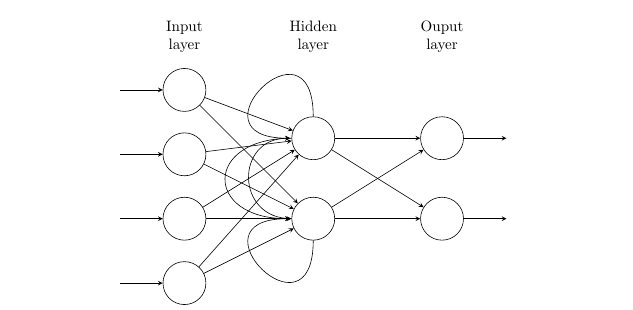
\includegraphics{Figures/RNN.png}
\[
\begin{cases}
h_{t} & =f\left(W_{xh}x_{t}+W_{hh}h_{t-1}+b_{h}\right)\\
o_{t} & =g\left(W_{hy}h_{t}+b_{o}\right)
\end{cases}
\]

\begin{itemize}
\tightlist
\item
  \(W_{xh}x_t\) : Input \(x_t\) is multiplied by weight matrix \(W_{xh}\) to extract information from the input
\item
  \(W_{hh}h_{t-1}\): Previous hidden state \(h_{t-1}\) is multiplied by weight matrix \(W_{hh}\) to extract information from ``memory''
\item
  Activation functions: \(f\) is usually \texttt{tanh} or \texttt{ReLU} and \texttt{g} is often \texttt{softmax}
\item
  \(b_h\) and \(b_o\) are biases.
\end{itemize}

\textbf{Advantages}

As we continue to emphasize, recurrent neural networks can model sequence of data -- either time-series or words in a sentence -- so that each sample is assumed to be dependent on the previous ones. From a modelling perspective, it is also very convenience since it can process input sequences of any length, and the model size does not increase for longer input sequence lengths. This is possible because computation for step \(t\) can use information from many steps back.

\textbf{Disadvantages}

One notable disadvantage is that training RNNs is slow since it is sequential and cannot be parallelized. In practice, it is difficult to access information from many steps back due to problems like vanishing and exploding gradients, which we discuss later in this section.

\hypertarget{training-rnns}{%
\subsection{Training RNNs}\label{training-rnns}}

\textbf{Backpropagation Through Time (BPTT)}

Backpropagation through time (BPTT) is simply backpropagation applied to sequence models with a hidden state and thus it is used to train recurrent neural networks. We relegate the details of the implementation to \href{https://d2l.ai/chapter_recurrent-neural-networks/bptt.html}{here}.

\hypertarget{vanishing-and-exploding-gradients}{%
\subsection{Vanishing and Exploding Gradients}\label{vanishing-and-exploding-gradients}}

\textbf{Vanishing Gradients}

In backpropagation, the gradients frequently become smaller and the new model weights end up being virtually identical to the old weights without any updates. As a result, the gradient descent algorithm never converges to the optimal solution. This is known as the problem of vanishing gradients.

Why does this happen? Vanishing gradients issue typically occur when using sigmoid or tanh activation functions in the hidden layer, which effectively compresses a large input space into a small output space. When the inputs become fairly small or fairly large, the derivatives become extremely close to zero and there is no gradient value to propagate back.

One obvious solution is to replace the activation function of the network by using ReLU instead of sigmoid. It keeps linearity for regions where sigmoid and tanh are saturated, thus responding better to gradient vanishing. Another solution is to consider a different architecture such as the LSTM, which we discuss later below. This post discusses other \href{https://datascience.stackexchange.com/questions/72351/how-to-prevent-vanishing-gradient-or-exploding-gradient}{potential changes}.

\textbf{Exploding Gradients}

If gradients get larger as the backpropagation progresses, we may end up with outsized weight updates, thereby leading to the divergence of the gradient descent algorithm.

Why does this happen? This problem happens because of weights and not because of the activation function. When the weight values are large, the derivatives will also be higher, thereby changing the weights significantly and preventing the gradient from converging.

A common solution is ``gradient clipping'' in which one may simply clip the parameter gradient element-wise before a parameter update or clip the norm of the gradient before a parameter update.

\hypertarget{applications}{%
\subsection{Applications}\label{applications}}

\textbf{Part-of-speech tagging}

The process of classifying words into their parts of speech and labeling them accordingly is known as part-of-speech tagging, or simply POS-tagging. \href{https://towardsdatascience.com/pos-tagging-using-rnn-7f08a522f849}{This post} provides an implementation using RNN.

\textbf{Text Generation}

Text generation is one obvious application of the RNN architecture. If we are training the neural network to predict the next character, it is called Character Level Model. Similarly, we can train the model to predict the next word, given a sequence of words called Word Level Models.

\hypertarget{lstm}{%
\section{LSTM}\label{lstm}}

Long Short-Term Memory RNNs (LSTMs) is a type of RNN proposed in 1997 as a solution to the vanishing gradients problem. As foreshadowed, its major strength is in capturing long-term dependencies in the sequence. \href{https://colah.github.io/posts/2015-08-Understanding-LSTMs/}{This post} provides a very detailed explanation for understanding LSTM networks. Here we provide the most essential details.

\hypertarget{basic-lstm-architecture}{%
\subsection{Basic LSTM Architecture}\label{basic-lstm-architecture}}

Recall that all RNNs have the form of a chain of repeating modules of neural network. In standard RNNs, this repeating module will have a very simple structure, such as a single tanh layer. LSTMs also have this chain like structure, but the repeating module has a different structure. Instead of having a single neural network layer, there are four, interacting in a very special way.

LSTM addresses the issues of the RNN by maintaining a cell state \((c_t)\), which is the state at any given time. This cell state is updated at each time step, and the output hidden state is derived from the input \((x_t)\), the previous hidden state (\(h_{t-1}\)), and the updated cell state \((c_t)\).

To read, erase, and write from the cell, there are also three corresponding gates. First is the \textbf{forget gate}, which is the first orange box on the left. It takes in the previous hidden state, the input and the learned weights to produce a number between 0 and 1. The second is the \textbf{input gate}, which consists of the next two orange boxes in the diagram. The first sigmoid layer decides which values to update, and the next tanh layer creates a vector of candidate values that can be added to the states.

Whether or not the update indeed happens is determined the by the last \textbf{output gate}, which consists of the last two orange boxes. The first sigmoid layer decides what parts of the cell state we're going to output, and then the cell state is put through the tanh layer and multiplied by the output of the sigmoid gate, so that we only output the parts we decided to. Note that the cell state also needs to be updated from \(c_{t-1}\) to \(c_t\). This is done at the horizontal arrow at the very top of the diagram.

\hypertarget{variations}{%
\subsection{Variations}\label{variations}}

One popular LSTM variant, introduced by Gers \& Schmidhuber (2000), is adding ``peephole connections.'' This means that we let the gate layers look at the cell state. Another variant is the Gated Recurrent Unit (GRU), which combines the forget and input gates into a single ``update gate.'' It also merges the cell state and hidden state, and makes some other changes. The resulting model is simpler than standard LSTM models, and has been growing increasingly popular. As GRU exposes the complete memory unlike the LSTM and is simpler, it is easier to modify and faster to train.

\hypertarget{other-extensions}{%
\section{Other Extensions}\label{other-extensions}}

\hypertarget{bidirectional-rnns}{%
\subsection{Bidirectional RNNs}\label{bidirectional-rnns}}

It is possible to make predictions based on future words by having the RNN model read through the corpus backwards. Such bi-directional RNN therefore maintains two hidden layers, one for the left-to-right propagation and another for the right-to-left propagation.

Since bidirectional RNNs require access to the entire input sequence, they are not applicable to language modeling in which only the left context is available. BERT is one such system built on bidirectionality.

\hypertarget{multi-layer-rnns}{%
\subsection{Multi-layer RNNs}\label{multi-layer-rnns}}

One can stack RNNs to construct a multi-layer RNNs. In such system, the hidden states from RNN layer \(i\) are the inputs to RNN layer \(i+1\). This allows the network to compute more complex representations.

High-performing RNNs are often multi-layer, ranging from 2 to 4 layers. This is actually not as deep as convolutional or feed-forward networks. Transformer-based networks such as BERT are usually deeper like 12 or 24 layers.

\hypertarget{attention-models-and-transformers}{%
\chapter{Attention Models and Transformers}\label{attention-models-and-transformers}}

\url{https://www.apronus.com/math/transformer-language-model-definition}

\hypertarget{attention}{%
\section{Attention}\label{attention}}

\hypertarget{basic-idea}{%
\subsection{Basic Idea}\label{basic-idea}}

In the context of language translation, the basic concept of attention is that each time the model predicts an output word, it only pays attention to some input words. Specifically, for each word in the output sentence, it will map the important and relevant words from the input sentence and assign higher weights to these words as shown in the figure below:

\begin{figure}
\centering
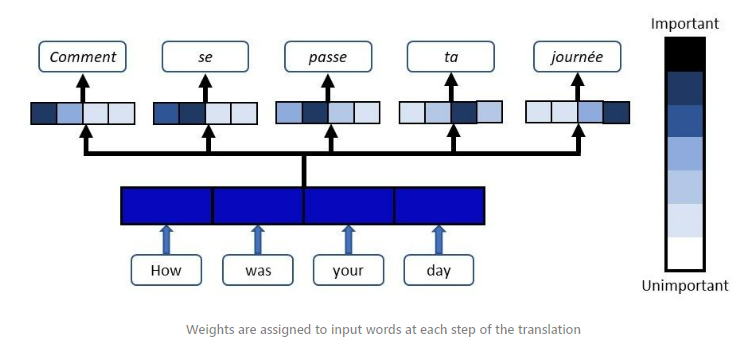
\includegraphics{Figures/transformers_01.png}
\caption{image-20220816201407808}
\end{figure}

In the traditional Seq2Seq model, we discard all the intermediate states of the encoder and use only its final states (vector) to initialize the decoder. The central idea behind attention is not to throw away these intermediate encoder states but to utilize all the states.

\hypertarget{steps-for-computing-attention}{%
\subsection{Steps for Computing Attention}\label{steps-for-computing-attention}}

\hypertarget{family-of-attention-mechanisms}{%
\subsection{Family of Attention Mechanisms}\label{family-of-attention-mechanisms}}

\begin{itemize}
\tightlist
\item
  There are different types of attention mechanisms: \url{https://lilianweng.github.io/posts/2018-06-24-attention/}
\end{itemize}

\hypertarget{self-attention}{%
\subsection{Self-Attention}\label{self-attention}}

Self-attention is equivalent to a generalized attention mechanism where the query, key, and values take the same input.

\hypertarget{transformers}{%
\section{Transformers}\label{transformers}}

\begin{itemize}
\tightlist
\item
  \url{https://www.lesswrong.com/s/nMGrhBYXWjPhZoyNL/p/McmHduRWJynsjZjx5}
\item
  \url{https://jalammar.github.io/illustrated-transformer/}
\end{itemize}

\hypertarget{overview-1}{%
\subsection{Overview}\label{overview-1}}

In its simplest form, a transformer takes in a sentence to translate and outputs a translated sentence:
\[
input \to transformer \to output
\]
The transformer consists of an encoder and a decoder:
\[
input \to encoder \to decoder \to output
\]
The encoder and the decoder consist of layers:

\begin{figure}
\centering
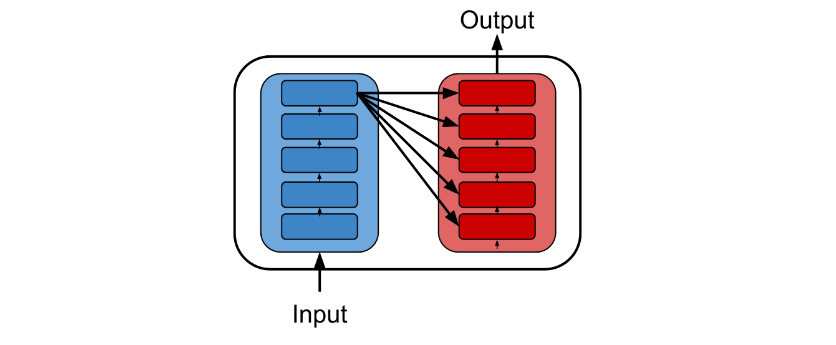
\includegraphics{Figures/transformers_02.png}
\caption{image-20220816203617350}
\end{figure}

\begin{itemize}
\tightlist
\item
  Notice that the sublayers are stacked linearly for both the encoder and the decoder, but the decoder takes an additional input: the output from the last encoder sub-layer.
\end{itemize}

Finally, each layer of the encoder and decoder take the following structure:

\begin{figure}
\centering
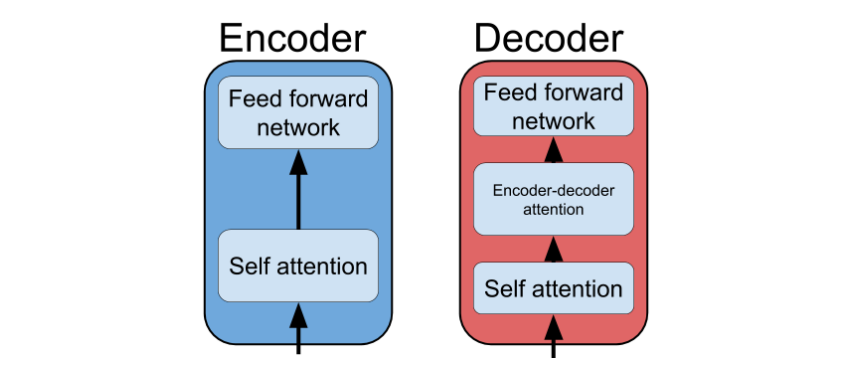
\includegraphics{Figures/transformers_03.png}
\caption{image-20220816204337867}
\end{figure}

\begin{itemize}
\tightlist
\item
  The encoder layer computes the self-attention and then feeds it into the feed-forward network.
\item
  The decoder layer is identical to the encoder layer with additional middle step: the encoder-decoder attention, which uses the information carried over from the last step of the encoder.
\end{itemize}

\hypertarget{step-1.-embedding}{%
\subsection{Step 1. Embedding}\label{step-1.-embedding}}

Before the input sentence can be fed into the architecture, it needs to be embedded via (1) word embedding and (2) positional encoding. Obviously, this embedding only happens in the bottom-most encoder.

\begin{itemize}
\tightlist
\item
  The word embedding is typically done through a pre-trained neural network instead of a simple one-hot encoding.
\end{itemize}

Positional encoding is also necessary because the transformer architecture does not include a default method for analyzing the order of words in the input sentence. In transformers, each position (index) is mapped to a vector, and hence the output of the positional encoding layer is a matrix where the \(i\)th row is a vector representing the \(i\)th token in the input sequence. This vector is then added to the original word embedding and fed into the very first encoder layer.

\begin{itemize}
\tightlist
\item
  See \href{https://jalammar.github.io/illustrated-transformer/}{this post} for details on the construction of this matrix.
\end{itemize}

\hypertarget{step-2.-self-attention-in-encoders}{%
\subsection{Step 2. Self-Attention in Encoders}\label{step-2.-self-attention-in-encoders}}

Self-attention is a layer that helps the encoder look at other words in the input sentence as it encodes a specific word. For example, suppose we are given the following input sentence: ``Simon called Manav because he felt overwhelmed.'' Self-attention allows the model to associate ``he'' with ``Simon'' and not ``Manav.''

For each word embedding vector, there is a vector of the attention layer. But we require the entire input sequence (i.e.~the list of words) for computing self-attention because (1) we need it to compute the weights (= normalized scores) and (2) we need to combine the weights with the value vectors, each of which is associated with each word input. \href{https://jalammar.github.io/illustrated-transformer/}{This post} describes the step-by-step process for computing self-attention very nicely, which is summarized below:

\begin{figure}
\centering
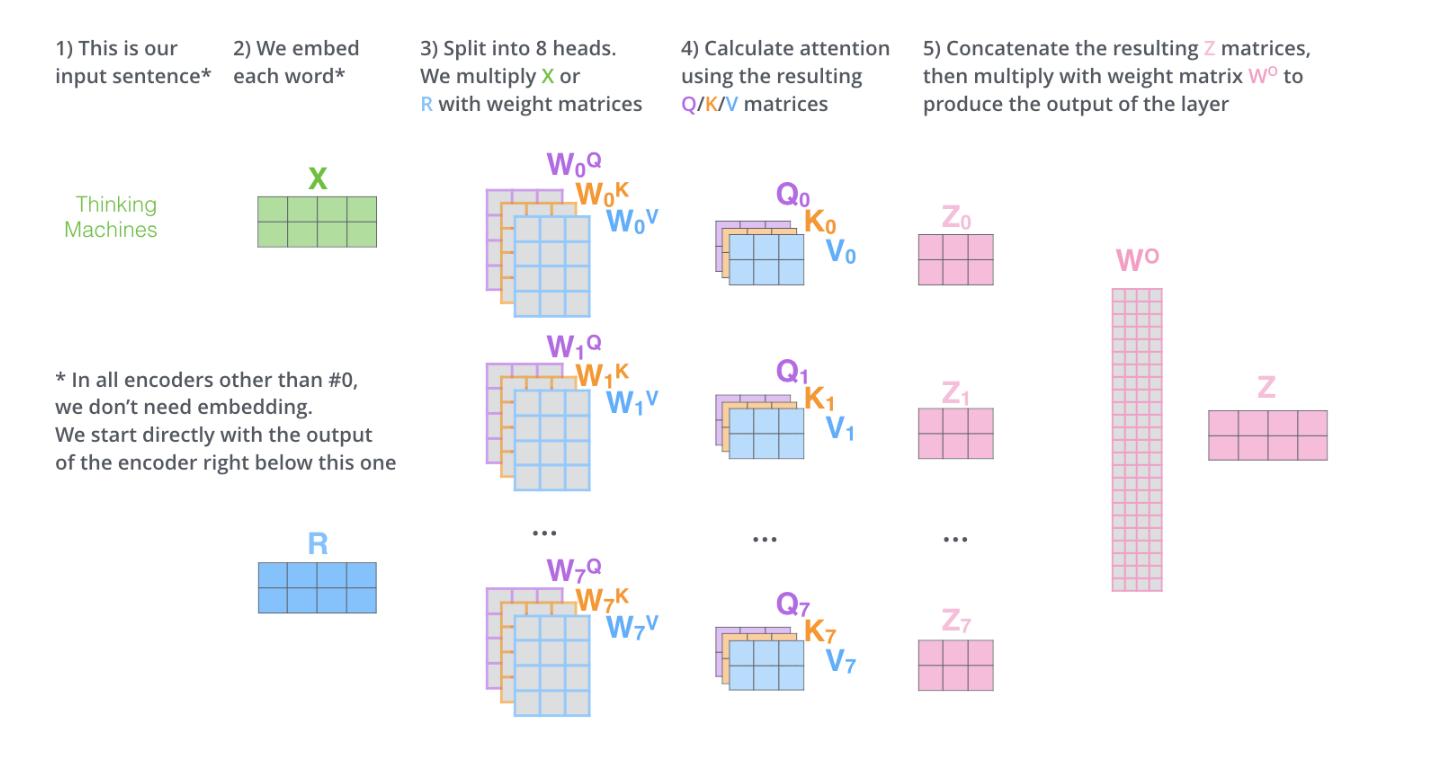
\includegraphics{Figures/transformers_04.png}
\caption{image-20220816214440095}
\end{figure}

\textbf{Step 1. Create Query, Key, and Value vectors}

The first step is to create, for each word, a Query vector, a Key vector, and a Value vector. These vectors are created by multiplying the embedding by three matrices that trained during the training process.

\begin{itemize}
\tightlist
\item
  Note that typically these new vectors are smaller in dimension than the embedding vector.
\end{itemize}

\textbf{Step 2. Compute the Score}

For each word, the score is is calculated by taking the dot product of the query vector with the key vector of the respective word. So for the word in position \(i\), the first score would be the dot product of \(q_i\) and \(k_1\) and the second score would be the dot product of \(q_i\) and \(k_2\).

\textbf{Step 3. Convert the Scores to Weights}

The scores are divided by \(\sqrt{d}\) where \(d\) is the dimension of the key vectors, which is intended to lead to more stable gradients. Then they are passed through a softmax operation so that the scores are converted to weights. The resulting softmax score determines how much each word will be expressed at this position.

\textbf{Step 4. Construct the self attention layer}

Each value vector is multiplied by the softmax score and then the weighted value vectors are summed to produce the output of the self-attention layer.

\textbf{Note: Multi-headed Attention}

\hypertarget{step-3.-self-attention-in-decoders}{%
\subsection{Step 3. Self-Attention in Decoders}\label{step-3.-self-attention-in-decoders}}

Similarly as before, the decoder passes its input into a multi-head self-attention layer. Unlike the one in the encoder, it is only allowed to attend to earlier positions in the sequence. This is done by masking future positions.

\hypertarget{step-4.-encoder-decoder-attention-in-decoders}{%
\subsection{Step 4. Encoder-Decoder Attention in Decoders}\label{step-4.-encoder-decoder-attention-in-decoders}}

This additional layer works like self-attention except that it combines two sources of inputs: the self-attention layer below it as well as the output of the encoder stack. \textbf{Importantly, the output from the encoder stack is passed to the value and key parameters, while the output of the self-attention module is passed to the query parameter.}

\hypertarget{pretrained-models-and-fine-tuning}{%
\chapter{Pretrained Models and Fine-Tuning}\label{pretrained-models-and-fine-tuning}}

In this section, we provide an ver

\hypertarget{bert}{%
\section{BERT}\label{bert}}

\hypertarget{gpt}{%
\section{GPT}\label{gpt}}

\hypertarget{other-useful-methods-for-textual-analysis}{%
\chapter{Other Useful Methods for Textual Analysis}\label{other-useful-methods-for-textual-analysis}}

\hypertarget{convolutional-neural-networks-cnns}{%
\section{Convolutional Neural Networks (CNNs)}\label{convolutional-neural-networks-cnns}}

\hypertarget{hidden-markov-models-hmms}{%
\section{Hidden Markov Models (HMMs)}\label{hidden-markov-models-hmms}}

\hypertarget{part-applications-in-econfinance}{%
\part*{APPLICATIONS IN ECON/FINANCE}\label{part-applications-in-econfinance}}
\addcontentsline{toc}{part}{APPLICATIONS IN ECON/FINANCE}

\hypertarget{sentiment-analysis}{%
\chapter{Sentiment Analysis}\label{sentiment-analysis}}

\hypertarget{part-code-snippets}{%
\part*{CODE SNIPPETS}\label{part-code-snippets}}
\addcontentsline{toc}{part}{CODE SNIPPETS}

\hypertarget{data-scraping}{%
\chapter{Data Scraping}\label{data-scraping}}

\hypertarget{data-cleaning}{%
\chapter{Data Cleaning}\label{data-cleaning}}

\hypertarget{word-tokenization}{%
\section{Word Tokenization}\label{word-tokenization}}

Tokenizers can easily become complex.

\hypertarget{implementing-tokenization}{%
\subsection{Implementing Tokenization}\label{implementing-tokenization}}

Several Python libraries implement tokenizers, each with its own advantages and disadvantages:

\begin{enumerate}
\def\labelenumi{\arabic{enumi}.}
\item
  spaCy---Accurate , flexible, fast, Python
\item
  Stanford CoreNLP---More accurate, less flexible, fast, depends on Java 8
\item
  NLTK---Standard used by many NLP contests and comparisons, popular, Python
\end{enumerate}

NLTK and Stanford CoreNLP have been around the longest and are the most widely used for comparison of NLP algorithms in academic papers.

\hypertarget{n-grams}{%
\subsubsection{N-Grams}\label{n-grams}}

An n-gram is a sequence containing up to n elements that have been extracted from a sequence of those elements, usually a string.

When a sequence of tokens is vectorized into a bag-of-words vector, it loses a lot of the meaning inherent in the order of those words. By extending your concept of a token to include multiword tokens, n-grams, your NLP pipeline can retain much of the meaning inherent in the order of words in your statements.

\hypertarget{techniques-for-normalizing-the-vocabulary}{%
\subsubsection{Techniques for Normalizing the Vocabulary}\label{techniques-for-normalizing-the-vocabulary}}

One can normalize the vocabulary so that tokens that mean similar things are combined into a single, normalized form. Doing so reduces the number of tokens you need to retain in your vocabulary and also improves the association of meaning across those different ``spellings'' of a token or n-gram in your corpus

\textbf{Case Folding}

Case folding is when you consolidate multiple ``spellings'' of a word that differ only in their capitalization. We can normalize the capitalization using list comprehension: \texttt{{[}x.lower()\ for\ x\ in\ tokens{]}}

\textbf{Stemming}

Another common vocabulary normalization technique is to eliminate the small mean- ing differences of pluralization or possessive endings of words, or even various verb forms. Stemming removes suffixes from words in an attempt to combine words with similar meanings together under their common stem. A stem isn't required to be a properly spelled word, but merely a token, or label, representing several possible spellings of a word.

It's important to note that stemming could greatly reduce the ``precision'' score for your search engine,
because it might return many more irrelevant documents along with the relevant ones.

Two of the most popular stemming algorithms are the Porter and Snowball stemmers. The Porter stemmer is named for the computer scientist Martin Porter. Porter is also responsible for enhancing the Porter stemmer to create the Snowball stemmer.

\begin{Shaded}
\begin{Highlighting}[]
\ImportTok{from}\NormalTok{ nltk.stem.porter}
\ImportTok{import}\NormalTok{ PorterStemmer}
\NormalTok{stemmer }\OperatorTok{=}\NormalTok{ PorterStemmer()}
\CommentTok{\textquotesingle{} \textquotesingle{}}\NormalTok{.join([stemmer.stem(w).strip(}\StringTok{"\textquotesingle{}"}\NormalTok{) }\ControlFlowTok{for}\NormalTok{ w }\KeywordTok{in} \StringTok{"dish washer\textquotesingle{}s washed dishes"}\NormalTok{.split()]))}
\end{Highlighting}
\end{Shaded}

\textbf{Lemmatization}

If you have access to information about connections between the meanings of various words, you might be able to associate several words together even if their spelling is quite different. This more extensive normalization down to the semantic root of a word---its lemma---is called lemmatization.

Lemmatization is a potentially more accurate way to normalize a word than stemming or case normalization because it takes into account a word's meaning. A lemmatizer uses a knowledge base of word synonyms and word endings to ensure that only words that mean similar things are consolidated into a single token.

So lemmatizers are better than stemmers for most applications. Stemmers are only really used in large-scale information retrieval applications (keyword search).

\begin{Shaded}
\begin{Highlighting}[]
\NormalTok{nltk.download(}\StringTok{\textquotesingle{}wordnet\textquotesingle{}}\NormalTok{)}
\ImportTok{from}\NormalTok{ nltk.stem }\ImportTok{import}\NormalTok{ WordNetLemmatizer}
\NormalTok{lemmatizer }\OperatorTok{=}\NormalTok{ WordNetLemmatizer()}
\NormalTok{lemmatizer.lemmatize(}\StringTok{"better"}\NormalTok{, pos}\OperatorTok{=}\StringTok{"a"}\NormalTok{) }\CommentTok{\# if POS is not specified, it assumes noun}
\end{Highlighting}
\end{Shaded}


  \bibliography{book.bib,packages.bib}

\end{document}
